\documentclass{article}
\usepackage[utf8]{inputenc}
\usepackage{titling}
\usepackage{german}
\usepackage{listings}
\usepackage{graphicx}
\usepackage{color}

\newcommand{\subtitle}[1]{%
  \posttitle{%
    \par\end{center}
    \begin{center}\large#1\end{center}
    \vskip0.5em}%
}
\title{Referat}
\subtitle{(AVLTree)}

\date{13. Dezember, 2017}
\author{Enes Kaya}

\begin{document}
  \maketitle
  \newpage

  Referat eingereicht im Rahmen der Vorlesung Algorithmen und Datenstrukturen\\*
  im Studiengang Angewandte Informatik (AI)\\*
  am Department Informatik\\*
  der Fakultät Technik und Informatik\\*
  der Hochschule für Angewandte Wissenschaften Hamburg\\*
  \newline
  Betreuender Prüfer: Prof. Dr. C. Klauck
  \newline
  Abgegeben am 12.12.2017
  
  \newpage
  \tableofcontents
  
  \newpage
  \section{Erklärung zur schriftlichen Ausarbeitung des Referates}
  
  Hiermit erkläre ich, dass ich diese schriftliche Ausarbeitung meines Referates selbstständig und ohne fremde Hilfe verfasst habe und keine anderen als die angegebenen Quellen und Hilfsmittel benutzt habe sowie die aus fremden Quellen (dazu zählen auch Internetquellen) direkt oder indirekt übernommenen Gedanken oder Wortlaute als solche kenntlich gemacht habe. Zudem erkläre ich, dass der zugehörige Programmcode von mir selbständig implementiert wurde ohne diesen oder Teile davon von Dritten im Wortlaut oder dem Sinn nach übernommen zu haben. Die Arbeit habe ich bisher keinem anderen Prüfungsamt in gleicher oder vergleichbarer Form vorgelegt. Sie wurde bisher nicht veröffentlicht.
  \newline
  \newline
  \newline
  Hamburg, den 12.12.2017
  
  \newpage
  \section{Aufgabenbeschreibung}
	Zu implementieren sei der abstrakte Datentyp AVL-Baum in der funktionalen Sprache Erlang. AVL Bäume sind höhen-balancierte Binär-Bäume. Durch diese Daten-Struktur, die zum Beispiel in Datenbanksystemen im Hintergrund für einen effizienten Zugriff auf Schlüssel gewährleistet, verhindert man u.a. dass Bäume bspw. zu Listen werden und so die erwartet Effizienz von Einfüge-, Lösch- und Such-Operationen verschlechtern. Das Suchen in einem AVL-Baum hat den Aufwand $O(log(n))$, dies wird später in den Tests und den Experimenten gezeigt.
	Diese Daten-Struktur wurde bereits 1962 von \textbf{A}delson-\textbf{V}elskii und \textbf{L}andis vorgeschlagen (Daher auch der Name AVL).
	
	\subsection{Geforderte Operationen}
	
	Um mit der Datenstruktur zu arbeiten werden folgende Operationen gefordert und implementiert:
	
	\begin{enumerate}
		\item $initBT()$: Gibt den initialen Baum zurück und dient als Konstruktor.
		\item $isEmptyBT(B)$: Prüft ob ein gegebener Baum $B$ leer ist und liefert einen Boolean
		\item $equalBT(B_1, B_2)$: Prüft rekursiv ob zwei gegebene Bäume strukturgleich sind und liefert einen Boolean
		\item $isBT(B)$: Prüft ob gegebener Baum B ein gültiger AVL-Baum ist und liefert einen Boolean
		\item $insertBT(B, N)$: Fügt rekursiv das Element N in B ein und liefert einen neuen Baum inklusive dem Element N. Führt eventuelle Rotations-Operationen aus.
		\item $deleteBT(B, N)$: Löscht rekursiv das Element N aus B und liefert einen neuen Baum exklusive dem Element N. Führt eventuelle Rotations-Operationen aus.
		\item $printBT(B, Filename)$: Erstellt eine Datei mit Anweisungen zum Drucken eines Binär-Baums mit Graphviz. 
	\end{enumerate}
	
	\subsection{Herangehensweise}
	
	Die Datenstruktur AVL-Baum baut auf die simplere ADT Baum auf. In der vorliegenden Ausarbeitung gehe ich daher besonders auf die Besonderheiten des AVL-Baums ein und lasse die Details zu Binär-Bäumen, soweit möglich, weg. Dieses Wissen über Binär-Bäume sei dem Leser dieser Ausarbeitung vorausgesetzt.

    % @TODO: Beschreiben was ein AVL Baum ist, die geforderten Operationen, die Ausgabe mittels .dot Dateien
  
  \subsection{TDD in Erlang}
  
  Um mögliches Refactoring, bzw. schnelles Testen der Implementierung zu gewährleisten wurde vor den Implementierungen ein EUnit-Test geschrieben (siehe Datei \textit{avltree\_tests.erl}). Für einen Blackbox-Test, sprich der Test der exportierten Schnittstellen, kann nun diese Datei kompiliert werden und mit EUnit ausgeführt werden.
  
\begin{lstlisting}[language=erlang]
c(avltree_tests).
c(avltree).
eunit:test(avltree).
\end{lstlisting}

	Für die Hilfsfunktionen wurden innerhalb des zu implementierenden Moduls (\textit{avltree.erl}) jeweils Test-Methoden hinzugefügt, welche dann auch beim EUnit Test-Aufruf durchlaufen.
  
  \newpage
  \section{Entwurf und Implementierung der Lösung}
  	Der abstrakte Datentyp AVL-Baum wird in Erlang mithilfe von Tupeln umgesetzt. Tupeln haben in Erlang eine feste Struktur und erlauben, im Vergleich zu Listen, weniger Operationen. Dadurch war schon von vornherein ein klarer Pfad notwendig, dem man bei der Implementierung befolgt. Zunächst wird festgelegt, dass das leere Tupel $\{\}$ den leeren Baum repräsentiert und somit für die Initialisierung (initBT) des AVL-Baums als Rückgabewert verwendet wird. 
    \newline
    Für den AVL-Baum wird nun folgende rekursive Struktur für einen Knoten bzw. den gesamten Baum festgelegt:
    
\begin{lstlisting}[language=erlang]
B = {Element, Hoehe, LinkerTeilbaum, RechterTeilbaum}.
\end{lstlisting}
    
    Ein Blatt sieht demnach so aus:
    
\begin{lstlisting}[language=erlang]
Blatt = {Element, Hoehe, {}, {}}
\end{lstlisting}
    
	An erster Stelle ist das eigentliche Element des Knotens, welches gemäß der Aufgabenstellung nur ganze Zahlen erlaubt. Die zweite Stelle ist eine positive, ganze Zahl, beginnend ab 1 für einen nicht-leeren Baum, die die Höhe des Knotens im gesamten Baum speichert. Die eigentliche Rekursion beginnt nun an 3. und 4. Stelle in dieser Datenstruktur, welche jeweils wieder einen Knoten/Teil-Baum speichern. Ein Blatt ist ein Knoten, mit der Höhe 1 und leeren Tupeln für den linken und rechten Teilbaum, wie im folgenden Beispiel veranschaulicht wird:

    \begin{lstlisting}[language=erlang]

B = { 5, 3, 
      { 2, 1, {}, {} }, 
      { 15, 2, 
        { 12, 1, {}, {} }, 
        {}
      }
    }.

    \end{lstlisting}
    
   	Welches den folgenden Baum darstellt:

	\begin{center}
   	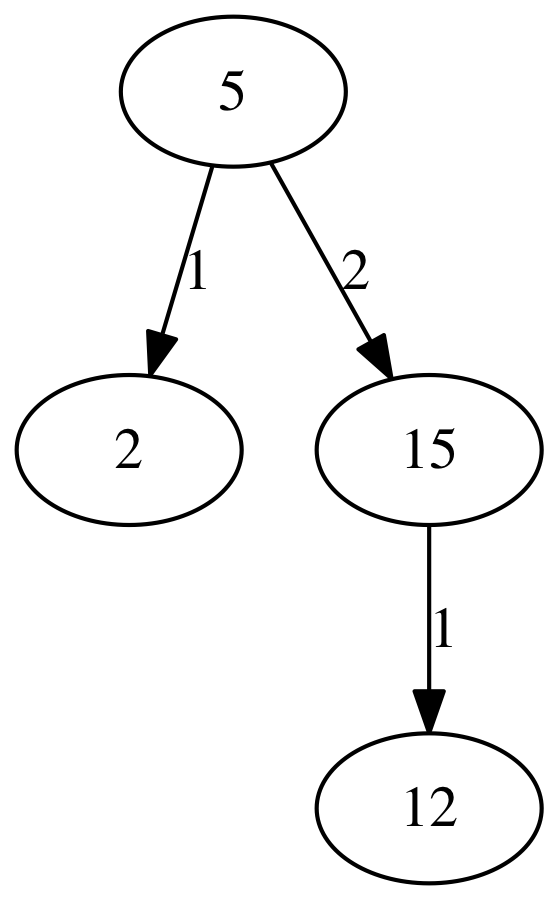
\includegraphics[height=3cm]{1.png}
	\end{center}

	Mit dieser Struktur und dem Pattern-Matching in Erlang ist es nun trivial, den Baum rekursiv zu durchlaufen. Die Struktur für den Baum steht nun fest, die Operationen, wie Einfügen und Löschen aus dem Baum werden im Nachfolgenden erläutert. Dabei liegt der Augenmerk immer in der Erhaltung der AVL-Bedingung.

	\subsection{AVL-Bedingung}
	\label{sec:avl-crit}

	Damit ein Baum ein AVL-Baum ist muss die AVL-Bedingung gelten. Dazu betrachtet man den \textbf{Balance-Faktor}, welcher definiert wird mit \\ $BF(t) = h(t_r) - h(t_l)$, wobei $t_l$ und $t_r$ jeweils den rechten und den linken Teilbaum von $t$ darstellen und $h(t)$ die Höhe eines Teilbaums ist.
	Ein Binär-Baum ist nun genau dann ein AVL-Baum wenn für alle Knoten in $t$ gilt: $BF(t) \in \{-1,0,1\}$. Ein Baum mit dem Balance-Faktor 0 nennt man ausgewogen. Mit $BF(t) < 0$ ist ein Baum links- und mit $BF(t) > 0$ rechtslastig.
	
	Für die Berechnung des Balance-Faktors in Erlang wird eine simple Funktion geschrieben:
	
	\begin{lstlisting}[language=erlang]
balanceFaktor({}) -> 0;
balanceFaktor({ _, _, {}, {}}) -> 0;
balanceFaktor({ _, _, {_, HL, _, _}, {}}) -> 0 - HL;
balanceFaktor({ _, _, {}, {_, HR, _, _}}) -> HR - 0;
balanceFaktor({ _, _, {_, HL, _, _}, {_, HR, _, _}}) -> 
  HR - HL.
	\end{lstlisting}
	
	Dank dem Pattern-Matching mit Tupeln in Erlang kann man so deklarativ den Balance-Faktor berechnen. \\
	Diese Funktion wird nun benutzt um eine eventuell benötigte Rotation zu erkennen und die richtige Rotation anzuwenden.
	
	\subsection{Rotationen}
	
	Beim Einfügen und beim Löschen in einen AVL-Baum muss vor und nach der Operation die AVL-Bedingung stets gelten. Um dies zu gewährleisten gibt es vier Wege eine Rotation an einem Knoten durchzuführen. Die \textit{Links-Rotation}, \textit{Rechts-Rotation}, \textit{Doppelt-Links-} und \textit{Doppelt-Rechts-Rotation}. Die Doppelt-Links-Rotation kann man auch als \textit{Rechts-Links-} und die Doppelt-Rechts-Rotation als \textit{Links-Rechts-Rotation} bezeichnen. 
	Welche Rotation angewendet werden muss kommt nun auf den Balance-Faktor eines Baums ein. Dazu wird eine Funktion geschrieben, die dies für einen Knoten feststellt (verkürzt):
	
	\begin{lstlisting}[language=erlang,numbers=left]
checkAndRebalance(Baum) ->
  BF_Ober = balanceFaktor(Baum),
  if
    BF_Ober == -2 ->
	  {_, _, TL, _} = Baum,
	  BF_Unter = balanceFaktor(TL),
	  if
	    BF_Unter == -1 -> rechtsRotation(Baum);
	    BF_Unter == 1 -> doppeltRechtsRotation(Baum)
	  end;
	BF_Ober == 2 ->
	  % ... gleich, nur fuer Links-Rotation.
  end.	
	\end{lstlisting}

	\textbf{Erläuterung}: In Zeile 2 wird zunächst der Balance-Faktor des Vater-Knotens berechnet (BF\_Ober). Falls dieser $-2$ beträgt, ist der gegebene Baum linkslastig und es muss eine (Doppelt-)Rechts-Rotation angewendet werden. Um nun zu entscheiden, welche Rotation angewandt wird wird der Balance-Faktor des linken Teilbaums bestimmt (Zeile 4 und Zeile 8-9).
	Das gleiche wird für den Fall durchgeführt, falls BF\_Ober gleich 2 ist. In diesem Fall wird dann natürlich eine (Doppel-)Links-Rotation angewandt.
	
	\subsubsection{Links- und Rechts-Rotation}
	
	Für die Rechts-Rotation wird der folgende Fall betrachtet:
	
	\begin{center}
   	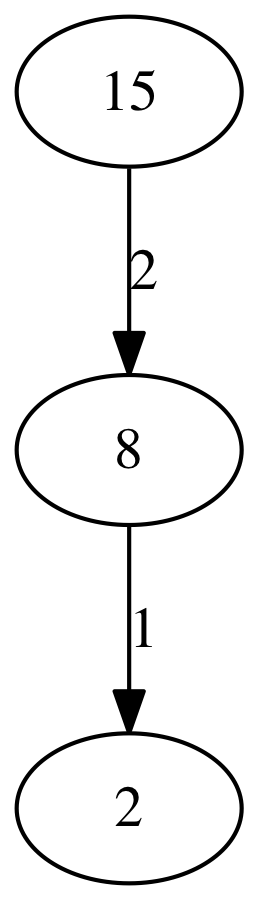
\includegraphics[height=3cm]{2.png}
	\end{center}
	
	Der Balance-Faktor für den Baum beträgt hier $0 - 2 = -2$. D.h. der Baum ist links-lastig. Der linke Teilbaum hat einen Balance-Faktor von $0 - 1 = -1$. Die \textit{checkAndRebalance} Methode führt für diesen Knoten nun eine einfache Rechts-Rotation aus.
	
	\begin{lstlisting}[language=erlang]
rechtsRotation({ E, _, L, R }) ->
  { LE, _, LL, LR } = L,
  NewRightNode = { E, berechneHoehe(LR, R), LR, R },
  NewNode = { LE,  berechneHoehe(LL, NewRightNode), LL, NewRightNode },
  NewNode.
	\end{lstlisting}
  
  	Der neue Rechte Knoten wird nun das Element E, mit der Höhe die sich aus dem rechten Teilbaum des linken Teilbaums und dem rechten Teilbaum des Ausgangs-Baums zusammensetzt. Hierzu wird auch die Hilfsfunktion \textit{berechneHoehe(L, R)} verwendet, die einfach nur $max(h(L), h(R)) + 1$ zurückgibt, wobei $h(B)$ die Höhe eines Baums B ist.
  	Der neue Knoten setzt sich nun zusammen aus dem Element des linken Teilbaums, dem linken Teilbaum des linken Teilbaums, und dem zuvor erwähnten neuen rechten Knoten.
  	
  	So führt nun die Eingabe für den oberen Baum mit dem Tupel 
  	\begin{lstlisting}
B = {15, 3, {8, 2, {2, 1, {}, {}}, {}}, {}}
  	\end{lstlisting}
	Zu der Ausgabe B1 mit 
	\begin{lstlisting}
B1 = {8, 2, {2, 1, {}, {}}, {15, 1, {}, {}}}
	\end{lstlisting}
  	
  	Der Baum ist nach dieser Operation wieder balanciert.
  	Auf die Links-Rotation wird jetzt nicht speziell eingegangen, da diese analog zur Rechts-Rotation auf dem rechten Teilbaum operiert.
  	
	\subsubsection{Doppel-Rotationen}
	
	Eine Doppel-Rechts- bzw. Links-Rotation ist eine Zusammensetzung aus einfachen Links- und Rechts-Rotationen, die man geschickt anwendet. So wird bei einem gegenen Baum $B$ und ihren Teilbäumen $B_L$ und $B_R$ die Doppelt-Rechts-Rotation wie folgt ausgeführt: Zunächst eine Links-Rotation auf $B_L$ und dann eine Rechts-Rotation auf den gesamten Baum $B$. Analog dazu wird bei einer Doppelt-Links-Rotation zunächst eine Rechts-Rotation auf $B_R$ und dann eine Links-Rotation auf auf den gesamten Baum $B$ angewandt.
	Im Code sieht das für die Doppelt-Rechts-Rotation dann folgendermaßen aus:
	
\begin{lstlisting}[language=erlang]
doppeltRechtsRotation({E, H, L, R}) ->
  rechtsRotation({ E, H, linksRotation(L), R }).
\end{lstlisting}
	
	\subsection{Prüfen, ob ein AVL-Baum vorliegt}
	
	Zur Überprüfung eines AVL-Baumes wird die rekursive Funktion $isBT(B)$ verwendet, welche $true$ für einen gültigen AVL-Baum liefert, $false$ sonst.
	
\begin{lstlisting}[language=erlang,numbers=left]
isBT(B) ->
  {E, H, L, R} = B,
  {LE, LH, _, _} = L,
  {RE, RH, _, _} = R,
  ValueCorrect = middle(E, LE, RE),
  HeightCorrect = (max(LH, RH) + 1) == H,
  BalanceIsValid = (abs(balanceFaktor(B)) =< 1),
  BalanceIsValid and
  HeightCorrect and 
  ValueCorrect and 
  isBT(L) and isBT(R).
\end{lstlisting}
	
	\textbf{Erläuterung}: \\
	Zeile 5: Es wird überprüft ob der Wert E des aktuellen Baums B zwischen dem Wert des linken und dem Wert des rechten Teilbaums von B liegt. Hierzu wird die Hilfsfunktion $middle$ benutzt.\\
	Zeile 6: Es wird überprüft, ob die Höhe des aktuellen Baums B korrekt ist. Die Höhe ist dann korrekt, wenn $max(h(B_L), h(B_R)) + 1 == h(B)$.\\
	Zeile 7: Es wird nun mithilfe der zuvor definierten Hilfs-Funktionen geschaut ob der Balance-Faktor des aktuellen Baums B im gültigen Bereich von -1 bis 1 liegt.\\
	Zeile 11: Der rekursive Aurfruf für jeweils den linken und den rechten Teilbaum gestartet wird gestartet.\\
	Ferner, und hier nicht zu sehen, gibt die Funktion für einen leeren Baum B $true$ zurück und beendet die Rekursion spätestens dort.
	
	\newpage
	
	\subsection{Einfügen in einen AVL-Baum}
	
	Das rekursive Einfügen in einen AVL-Baum muss dafür sorgen, dass zusätzlich zum Einfügen wie in einen Binär-Baum die AVL-Bedingung erhalten bleibt.

\begin{lstlisting}
insertBT(B, N) -> B.
\end{lstlisting}

	\textbf{Objektmengen}: N = Einzufügendes Element, E = Element des aktuellen Knotens, B = (Teil-)Baum
	
	\begin{enumerate}
		\item Prüfe, ob einzufügendes Element N vom Typ \textit{Integer} ist. Falls ja, mache weiter. Falls nein, kann hier abgebrochen werden.
		\item Falls $N > E$, wird das Element rekursiv in den rechten Teilbaum $B_R$ von B eingefügt: $insertBT(B_R, N)$
		\item Prüfe, ob sich die Höhe verändert hat nach der vorherigen Einfüge-Operation. Falls ja, prüfe an dem aktuellen Knoten die AVL-Bedingung und führe evtl. eine Rotation durch. Falls nein, und die Höhe hat sich nicht geändert ist auch keine Rebalancierung notwendig. 
		\item (Analog für $N < E$)
	\end{enumerate}
	
	Die Rekursion wird aufgelöst, sobald das Element an einen Teil-Baum als Blatt hinzugefügt worden ist. Hierzu wird die Funktion $insertBT(\{\}, N)$ definiert, welche nur einen neuen Baum mit N als Element, der Höhe 1 und jeweils leerem linken und rechten Teilbäumen zurückgibt.
	
	\newpage
	\subsection{Löschen aus einem AVL-Baum}

	Das Löschen eines Knoten aus einem AVL-Baum funktioniert folgendermaßen:
	\\\\
	\textbf{Objektmengen}: D = Zu löschendes Element, B = Baum
	
	\begin{enumerate}
		\item Gehe rekursiv zum zu löschenden Knoten durch Traversion von $B$
		\item Knoten wurde gefunden: Ersetze den gefundenen Knoten mit dem größten Element aus dem linken Teilbaum bzw., falls linker Teilbaum leer, mit dem kleinsten Element aus dem rechten Teilbaum und lösche diesen (rekursiv) Knoten
		\item Falls der zu löschende Knoten ein Blatt ist, lösche es
	\end{enumerate}
	
	Der Quell-Code dazu sieht so aus:\newline
	
\begin{lstlisting}[language=erlang,numbers=left]
deleteBT({E, H, L, R}, D) ->
  if
    D > E -> 
      NewRight = deleteBT(R, D),
      NewHeight = berechneHoehe(L, NewRight),
      checkAndRebalance({ E, NewHeight, L, NewRight });
    D < E ->
      NewLeft = deleteBT(L, D),
      NewHeight = berechneHoehe(NewLeft, R),
      checkAndRebalance({ E, NewHeight, NewLeft, R });
    D == E ->
      if
        H == 1 -> {};
        not LeftEmpty ->
          BiggestLeftChild = findBiggest(L),
          NewLeft = deleteBT(L, BiggestLeftChild),
          NewHeight = berechneHoehe(NewLeft, R),
          checkAndRebalance({BiggestLeftChild, NewHeight, NewLeft, R});
        not RightEmpty ->
          SmallestRightChild = findSmallest(R),
          NewRight = deleteBT(R, SmallestRightChild),
          NewHeight = berechneHoehe(L, NewRight),
          checkAndRebalance({ SmallestRightChild, NewHeight, L, NewRight })
      end;
    true -> {E, H, L, R }
  end.
\end{lstlisting}

  	\newpage
  	\section{Testumgebung}
  
  	\newpage
  	\section{Quellen}

\end{document}








